\documentclass{beamer}
\usepackage[utf8]{inputenc}

\usetheme{Madrid}
\usecolortheme{default}
\usepackage{txfonts}
\usepackage{listings}
\usepackage{adjustbox}
\usepackage{tabularx}
\usepackage{lmodern}
\usepackage{circuitikz}
\usepackage{tikz}

\usepackage{gvv}
\usepackage{cite}
\usepackage{amsmath,amssymb,amsfonts,amsthm}
\usepackage{algorithmic}
\usepackage{graphicx}
\usepackage{textcomp}
\usepackage{xcolor}
\usepackage{txfonts}
\usepackage{listings}
\usepackage{enumitem}
\usepackage{mathtools}
\usepackage{gensymb}
\usepackage{comment}
\usepackage{tkz-euclide} 
\usepackage{listings}                                      
\def\inputGnumericTable{}                                
\usepackage{color}                                            
\usepackage{array}                                            
\usepackage{longtable}
\usepackage{multicol}
\usepackage{calc}                                             
\usepackage{multirow}                                         
\usepackage{hhline}                                           
\usepackage{ifthen}

\setbeamertemplate{page number in head/foot}[totalframenumber]

\usepackage{tcolorbox}
\tcbuselibrary{minted,breakable,xparse,skins}



\definecolor{bg}{gray}{0.95}
\DeclareTCBListing{mintedbox}{O{}m!O{}}{%
  breakable=true,
  listing engine=minted,
  listing only,
  minted language=#2,
  minted style=default,
  minted options={%
    linenos,
    gobble=0,
    breaklines=true,
    breakafter=,,
    fontsize=\small,
    numbersep=8pt,
    #1},
  boxsep=0pt,
  left skip=0pt,
  right skip=0pt,
  left=25pt,
  right=0pt,
  top=3pt,
  bottom=3pt,
  arc=5pt,
  leftrule=0pt,
  rightrule=0pt,
  bottomrule=2pt,
  toprule=2pt,
  colback=bg,
  colframe=orange!70,
  enhanced,
  overlay={
    \begin{tcbclipinterior}
    \fill[orange!20!white] (frame.south west) rectangle ([xshift=20pt]frame.north west);
    \end{tcbclipinterior}},
  #3,
}
\lstset{
    language=C,
    basicstyle=\ttfamily\small,
    keywordstyle=\color{blue},
    stringstyle=\color{orange},
    commentstyle=\color{green!60!black},
    numbers=left,
    numberstyle=\tiny\color{gray},
    breaklines=true,
    showstringspaces=false,
}

\title 
{4.7.22}
\date{September 30, 2025}


\author 
{Sai Sreevallabh - EE25BTECH11031}



\begin{document}


\frame{\titlepage}
\begin{frame}{Question}
In what direction should a line be drawn through the point $\brak{1,2}$ so that its point of intersection with the line $x+y=4$ is at a distance $\sqrt{63}$?\\
\end{frame}



\begin{frame}{Theoretical Solution}
The given point is $\vec{P} = \myvec{1\\2}$.\\

The given line can be represented as $\vec{n}^\top\vec{x} = c$, where 
\begin{align}
    \vec{n} = \myvec{1\\1} \ \ c = 4
\end{align}\\

A parametric point on the line passing through the point $\vec{P}$ is given by 
\begin{align}
    \vec{r} = \vec{P} + \lambda\vec{m}
\end{align}

where $\vec{m} = \myvec{1\\m}$\\

\end{frame}

\begin{frame}{Theoretical Solution}

Plugging in the parametric form of the point in the line equation, we get: 

\begin{align}
    \vec{n}^\top\brak{\vec{P+\lambda\vec{m}}}\  =&\  c\\
    \lambda \ =&\  \frac{c-\vec{n}^\top\vec{P}}{\vec{n}^\top\vec{m}}
\end{align}\\

Replacing this value of $\lambda$ in the equation of the parametric point, we get it to be
\begin{align}
    \vec{r} = \vec{P} + \brak{\frac{c-\vec{n}^\top\vec{P}}{\vec{n}^\top\vec{m}}}\vec{m}
\end{align}\\

\end{frame}

\begin{frame}{Theoretical Solution}
Substituting the values, we get

\begin{align}
    \sqrt{63} =& \abs{\frac{4-3}{1+m}}\sqrt{1+m^2}
\end{align}\\

Squaring on both sides:
\begin{align}
    63 =& \frac{1+m^2}{\brak{1+m}^2}
\end{align}
\end{frame}

\begin{frame}{Theoretical Solution}
This is an equation in $m$. Upon solving this equation, we get:

\begin{align}
    m = \frac{-63 \pm 5\sqrt{5}}{62}
\end{align}

$\therefore$ The direction vector $\vec{m}$ can take two values:
\begin{center}
    $\vec{m} = \myvec{1\\\frac{-63 + 5\sqrt{5}}{62}} \ \ \text{or} \ \ \vec{m} = \myvec{1\\\frac{-63 - 5\sqrt{5}}{62}}$
\end{center}
\end{frame}


\begin{frame}[fragile]
    \frametitle{C Code - Function to Find y Coordinate of P}

    \begin{lstlisting}

#include <stdio.h>
#include <math.h>

void solve_quad(double a, double b, double c, double sols[2]){
   
    double D = b*b - 4*a*c;
   
    sols[0] = (-b+pow(D,0.5))/(2*a);
    sols[1] = (-b-pow(D,0.5))/(2*a);
   
}
    \end{lstlisting}

\end{frame}

\begin{frame}[fragile]
    \frametitle{Python Code - Using Shared Object}
    \begin{lstlisting}
import ctypes
import numpy as np
import matplotlib.pyplot as plt


c_lib = ctypes.CDLL("./code.so")

c_lib.solve_quad.argtypes = [ctypes.c_double, ctypes.c_double, ctypes.c_double, ctypes.c_double*2]

a,b,c = 31.0, 63.0, 31.0
P = np.array([1,2])
sol = (ctypes.c_double*2)(0.0,0.0)

c_lib.solve_quad(a,b,c,sol)


\end{lstlisting}
\end{frame}

\begin{frame}[fragile]
    \frametitle{Python Code - Using Shared Object}
    \begin{lstlisting}

m1 = sol[0]
m2 = sol[1]

t = (2+m1)/(m1+1)
k = (2+m2)/(m2+1)

A = np.array([t,4-t], dtype = np.double)
B = np.array([k, 4-k], dtype = np.double)

plt.plot([-5,8], [9,-4], c='black', label = "$x+y=4$")
plt.plot([P[0],A[0]], [P[1], A[1]], c='green')
plt.plot([P[0],B[0]], [P[1], B[1]], c='red')


\end{lstlisting}
\end{frame}

\begin{frame}[fragile]
    \frametitle{Python Code - Using Shared Object}
    \begin{lstlisting}
    
plt.scatter([1,t,k],[2,4-t,4-k])
plt.annotate(
        "P(1,2)",
        xy=(1,2),
        xytext = (-15,-15),
        textcoords = "offset points"
        )


\end{lstlisting}
\end{frame}



\begin{frame}[fragile]
    \frametitle{Python Code - Using Shared Object}
    \begin{lstlisting}
    
ax = plt.gca()
ax.spines['top'].set_color('none')
ax.spines['left'].set_position('zero')
ax.spines['right'].set_color('none')
ax.spines['bottom'].set_position('zero')
plt.xlabel('$x$')
plt.ylabel('$y$')
plt.legend(loc='best')
plt.grid() 
plt.axis('equal')

plt.savefig("../Figs/plot(py+C).png")

plt.show()

\end{lstlisting}
\end{frame}

\begin{frame}{Plot-Using Both C and Python}
    \centering
    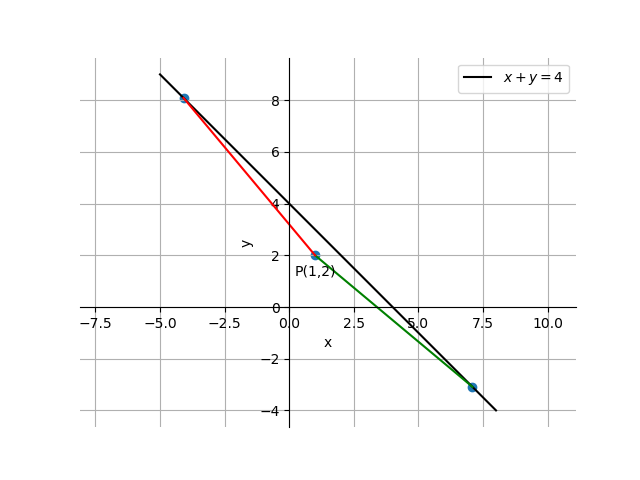
\includegraphics[width=\columnwidth, height=0.8\textheight, keepaspectratio]{Figs/plot(py+C).png}     
\end{frame}

%-------End of Python+C-------------


\begin{frame}[fragile]
    \frametitle{Python Code}
    \begin{lstlisting}
import numpy as np
import numpy.linalg as LA
import matplotlib.pyplot as plt

a,b,c = 31,63,31
P = np.array([1,2])

roots = np.roots([a,b,c])

t = (2+roots[0])/(roots[0]+1)

A = np.array([t,4-t], dtype = np.double)

k = (2+roots[1])/(roots[1]+1)

B = np.array([k, 4-k], dtype = np.double)

\end{lstlisting}
\end{frame}

\begin{frame}[fragile]
    \frametitle{Python Code}
    \begin{lstlisting}

plt.plot([-5,8], [9,-4], label = "$x+y=4$")
plt.plot([P[0],A[0]], [P[1], A[1]])
plt.plot([P[0],B[0]], [P[1], B[1]])

plt.scatter([1,t,k],[2,4-t,4-k])
plt.annotate(
        "P(1,2)",
        xy=(1,2),
        xytext = (-15,-15),
        textcoords = "offset points"
        )


\end{lstlisting}
\end{frame}

\begin{frame}[fragile]
    \frametitle{Python Code}
    \begin{lstlisting}
ax = plt.gca()
ax.spines['top'].set_color('none')
ax.spines['bottom'].set_position('zero')
ax.spines['right'].set_color('none')
ax.spines['left'].set_position('zero')
plt.xlabel('x')
plt.ylabel('y')
plt.legend(loc='best')
plt.grid()
plt.axis('equal')

plt.savefig("../Figs/plot(py).png")
plt.show()


    \end{lstlisting}
\end{frame}


\begin{frame}{Plot-Using Python only}
    \centering
    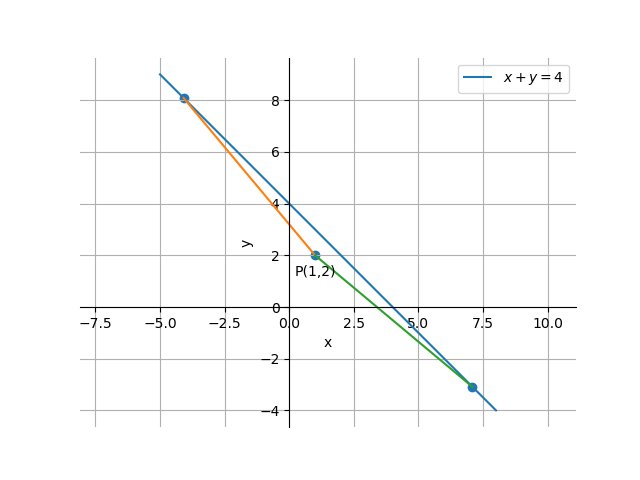
\includegraphics[width=\columnwidth, height=0.8\textheight, keepaspectratio]{Figs/plot(py).png}     
\end{frame}


\end{document}
